\section{Faster R-CNN}  \label{sec:faster_rcnn}

\begin{figure}[!ht]
    \centering
    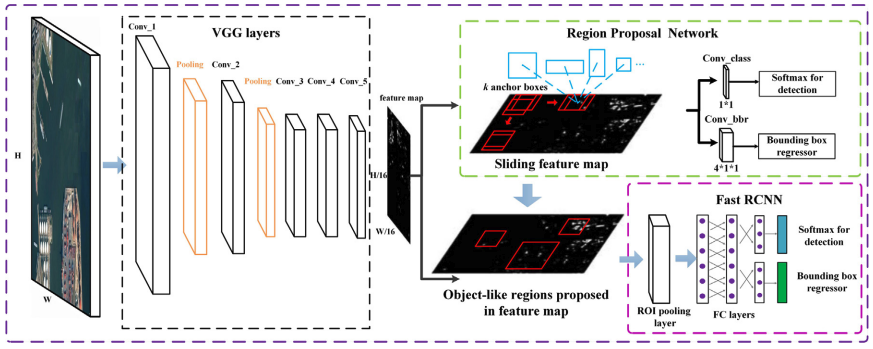
\includegraphics[width=5in]{figures/faster_rcnn_archite.png}
    \caption{Faster R-CNN overall architecture \cite{faster_rcnn_architecture_fig}} \label{fig:faster_rcnn_archite}
\end{figure}

In 2016, the object detection Faster R-CNN model was proposed as an improvement over the Fast R-CNN model. The Faster R-CNN model is composed of two modules . The first module is responsible for generating RoIs with a CNN. The second module is a classification CNN. At its core, Faster R-CNN is a Fast R-CNN model with a region proposal network (RPN) [Fig. \ref{fig:faster_rcnn_archite}]. In another words, the RPN generate RoIs, then Fast R-CNN takes these generated RoIs as input and generate bounding box locations and class scores. Through testing with different datasets like PASCAL VOC and COCO, Fast R-CNN with RPN as a region proposal method consistently achieved higher accuracy scores compared to when generating RoIs with the selective search algorithm. As an example, when testing the Fast R-CNN based on VGG-16 on the combined dataset of PASCAL VOC 2007 and 2012, the use of RPN to generate RoIs resulted in a higher mAP score of 73.2\% compared to the Selective Search algorithm, which achieved an mAP score of 70\% \cite{faster_rcnn_2015}.

\subsection{Region Proposal Network (RPN)}  \label{subsec:rpn}
The Region Proposal Network (RPN) is a fully connected convolutional network engineered to propose regions of interest (RoIs) regardless of object scales and aspect ratios. RPN accepts image of any size as input and outputs several bouding boxes, each with a score representing the possibility of an object residing in the box under consideration. The main advantage of RPN over Selective Search is, while Selective Search is implemented in CPU, RPN is implemented in GPU. Utilizing the computation power of GPU instead of CPU help boost the performance of region proposal tremendously. Moreover, since models like Fast R-CNN also use GPU and convolutional layers to generate detection, RPN can share computation with Fast R-CNN through a multi-task loss. Consequently, reduce the computational power needed for generating RoIs to almost none when added on top of the computation already needed by the object detection module. As a comparison, RPN able to generate RoIs in 0.01 second oppose to 2 seconds with Selective Search, while achieving higher accuracy score overall \cite{faster_rcnn_2015}. Furthermore, unlike Selective Search, which is a fixed algorithm and not trainable, RPN is a learnable neural network. Thus the performance will increase when more data is fed and/or a deeper network is being used. 

\begin{figure}[!ht]
    \centering
    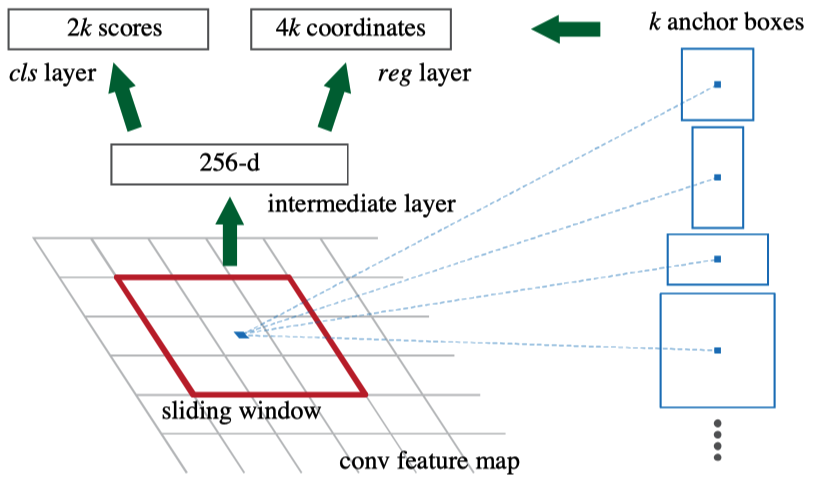
\includegraphics[width=3in]{figures/rpn_anchor.png}
    \caption{Region Proposal Network (RPN) \cite{faster_rcnn_2015}} \label{fig:faster_rcnn_anchor}
\end{figure}

The RPN model can be thought of as two stage process. In the first stage, RPN applies a CNN over the inputted image and generates a feature map for the entire image. The same operation is taken in the first stage of Fast R-CNN. Thus, Faster R-CNN can have a CNN to generate the image feature map, and then the image feature map proceeds as input for the second stage of RPN and Fast R-CNN. Thereby sharing computation between the two modules of Faster R-CNN. In the second stage, RPN slides a $3 \times 3$ convolutional layer, then branched to two siblings $1 \times 1$ layers. The first branch is a bounding box regressor (named $reg$) that generates a set of four values representing the coordinate of the bounding box. The second branch is a classifier (named $cls$) that produces a score for the probability that the object is in the window. At each sliding window location, RPN create an anchor at the center of the window. Then, with 3 different scaling factors and 3 different aspect ratios, RPN generate 9 new proposals with the anchor at the center [Fig. \ref{fig:faster_rcnn_anchor}]. Since RPN behavior is based on the sliding window technique, it exhausted all possible locations, and with the use of 9 different sizes and aspect ratios, RPN gains the translation invariant property. That is, RPN is guaranteed to be able to generate the object's location even if some translation operation is performed on the object.

Similar to Fast R-CNN, the RPN model is trained end-to-end with a multi-task loss. The multi-task loss is derived based on the classification loss and regression loss across anchor points from the $cls$ and $reg$ branches, respectively. The classification loss evaluates the accuracy of classifying objects versus non-objects, while the regression loss assesses the accuracy of predicting bounding box coordinates. If RPN samples all anchor points, then the model will favor negative false as the majority of RPN's generated predicted bounding boxes does not overlap with any truth box. To resolve this problem, RPN employs a sample-dropping technique, then randomly selects 256 samples from the remaining samples to help balance positive and negative samples \cite{faster_rcnn_2015}. For sample dropping, RPN marks all predicted boxes with over 70\% overlap with any truth box as positive and those with less than 30\% overlap as negative. Predicted boxes that are neither marked as positive nor negative are dropped. Then, RPN applies non-maximum suppression (NMS) to reduce the remaining samples, since the generation of 9 proposals at each anchor location may result in highly overlapping boxes. During NMS, any two proposed bounding boxes that overlap by more than 70\% with each other are compared, and the one with a higher $cls$ score is kept while the other is dropped. With that being said, the RPN training process consists of three steps. In step one, the pre-trained VGG-16 model is used to initialize the shared CNN, and weight values are randomly assigned to the RPN's unique layers. Next, RPN is trained with the stochastic gradient descent (SGD) method, using mini-batches of 256 predicted bounding boxes from the remaining proposals after sample-dropping described above. In the last step, The model uses the previously described multi-task loss during each iteration to perform backpropagation.

\subsection{Training}  \label{subsec:faster_rcnn_training}
Although it is possible to train the RPN and Fast R-CNN components independently in Faster R-CNN as described previously. However, because the network learns significantly differently for object proposal and classification task, optimizing the shared convolutional layers one task may not fully optimize them for the other task. To address this issue, Faster R-CNN employs a four-step alternative training procedure. Faster R-CNN trains an RPN model separately in the first phase as described previously. Faster R-CNN trained a separate Fast R-CNN network in the second phase, which uses the RoIs generated by RPN in the first step as input for the classification task. Once the second phase is completed, Faster R-CNN trains the unique layer to RPN using the trained Fast R-CNN. This means that all Fast R-CNN layers are being fixed during this step, while the $3 \times 3$ convolutional layer and two siblings $1 \times 1$ layers unique to RPN are being trained. In the last phase, Faster R-CNN fixed the shared convolutional layers and layers specific to the RPN, so training occurs on Fast R-CNN's unique layers. This 4-step alternative training process is carried through each minibatch of SGD. The author of Faster R-CNN mentions two other shared schemes, approximate joint training, and non-approximate joint training, in addition to the alternative training scheme \cite{faster_rcnn_2015}. Unfortunately, both methods are impeded by issues beyond this study's scope; therefore, we will not go into depth.

By combining the VGG16 and RPN with Fast R-CNN model and trained with the union training set of PASCAL VOC 2007 + 2012, Faster R-CNN, using the top 300 proposals ranked by RPN's $cls$ branch, achieved an mAP score of 73.2\% when tested on the PASCAL VOC 2007 test set. This is 3.2\% higher than when replacing RPN with Selective Search, which generated 2000 proposals for Fast-RCNN. Moreover, when using only the top ranked 100 proposals, Faster R-CNN still achieved an mAP score of 55.1\%, indicating that RPN's top ranked proposals are highly accurate and that the $cls$ branch is important. Furthermore, Faster R-CNN can process 5 images per second, which is 10 times faster than the processing rate achieved by Fast R-CNN with Selective Search, which is 0.5 images per second \cite{faster_rcnn_2015}. 

Faster R-CNN has been a significant breakthrough in the field of object detection. It achieved a much higher mAP score while maintaining a near real-time processing rate compared to its predecessor, Fast R-CNN. However, it is important to note that Faster R-CNN is limited to performing object detection and does not support instance segmentation. Instance segmentation involves not only detecting objects in an image but also segmenting each object at a pixel level. Additionally, Faster R-CNN still suffers from the quantization issue caused by the RoI pooling layer, as described in the previous section. In the next section, we will discuss Mask R-CNN, which adds instance segmentation capabilities to Fast R-CNN and resolves the quantization issue.